\documentclass[10pt,twocolumn]{article}
\usepackage{times}
\usepackage{url}
\usepackage{graphicx} 
\usepackage{subfigure}
\usepackage{float}
\usepackage{booktabs}
\usepackage{multirow}
\usepackage{diagbox}

\usepackage{algorithm}
\usepackage{algorithmic}


% do not change these values
\baselineskip 12pt
\textheight 9in
\textwidth 6.5in
\oddsidemargin 0in
\topmargin 0in
\headheight 0in
\headsep 0in

\setlength{\abovecaptionskip}{0pt}
\setlength{\belowcaptionskip}{10pt}

\begin{document}

\title{ClaTex: LaTeX as a Service on the Cloud}
\author{John Doe$^1$ and Jane Monroe$^2$ \\
\small {\em  $^1$Dept. Cloud, Cloud University \quad
          $^2$Cloud National Labs} \\ [2mm]
\small Submission Type: Research
}
\date{}
\maketitle

\begin{abstract}
The time has come to offer LaTeX on the cloud.
\end{abstract}

\section{Introduction}
Virtualization is a basic technology for the cloud computing. The growing awareness of the advantage provided by virtualization technology is brought about by economic factors of scarce resouces, government regulation and more competition.

Virtualizaton provides the ability of consilidation for virtual machines(VM). Mutiple VMs share the same physical machine without any interference of each other. However, virtualization providers suppose VMs on the same physical machine are unlikely to use up the whole memory at the same time. So VMs are often configured more memory in total than the capacity of the physical machine. But on the worse case, VMs compete with each other leading to shortness of memory resources. Other technology like migration also provided by virtualization must start up soon. Otherwise, some VMs may suffer memory starvation and lose the performance of the application on top of that.

With the development of hardware, a typical host machine in a datacenter now packs tens to hundreds of VMs in order to maximize resouce utilization. VMware ESXi hypervisor has increased the number of VMs supported per host from 32 to 1024 in recent years\cite{vmware}. Memory as shared resources needs to be allocated on demand in order to full resouce utilization but still the minimum QoS has to be guaranteed since users buy for it. VM providers should be able to cope with the situation when memory increases suddenly.

In virtualization environment, guest OS is transparent to the underlying hypervisor. There are only some basic monitoring statics exposed to hypervisor such as VSZ and RSS in linux system. VSZ and RSS are coarse-grained statics which did not reflect the memory usage in a certern period. In the past, working set theory\cite{wss} has been widely used to capture applications' memory needs. Working sets is defined as the set of all pages accessed by a process over a given epoch. However, working set doesn't relate directly to the performance of an application. For example, if an application scans 100 pages sequentially. In a short period, the working set is 100 pages. But allocating 1 page or 100 pages gives the same memory hit ratio because the miss ratio is always 100\%. MRC is the alternative to working set theory. It plots the miss rate against given physical memory. MRC may differ every second reflecting the memory requirement changes of the application which gives us a hint to dynamic allocate more or reclaim spare memory in order to utilize the host machine's resources better.

MRC theroy is a general method to curve the miss rate and each part of the memory hierachy in computer storage including cache, memory and etc. Recently many research focus on the cache MRC construction. Centaur\cite{Koller2015Centaur} implements host-side SSD cache partition for VMs that provides both lower cache miss rate and better performance isolation and performance control for VM workloads. Like Centaur, Multi-Cache\cite{Rajasekaran2016Multi} presents multiple cache management on a set of storage devices and intelligently manages how caches are shared by competing VMs. Moirai\cite{Stefanovici2015Software} presents a tenant- and workload-aware system that allows data center providers to control their distributed caching infrastructure. 



\section{Motivation}
Since the needs of oversold of memory and still high performance ensurance of VMs. Memory prediction is still a valuable research area especially on the area of cloud computing. To relat the memory size and the performance, a traditional approach is to use page miss ratio curve(MRC). MRC shows the miss rate under given memory size. A way to track MRC is to use LRU stack algorithm\cite{Mattson1970Evaluation}. But the time complexity and space usage is high which makes it hard to track MRC online.

Recently there are some breakthroughts to track MRC in efficient ways. Counter Stacks\cite{Wires2014Characterizing} use probabilistic counters to estimate approximate MRC at a fraction of the cost of traditional techniques. SHARDS\cite{shards} simply uses sampling to reduce the size of input trace. Both approachs reduces the time complexity and space cost in constructing MRC and makes it possible to online tracking. AET\cite{aet} descrbes a new kinetic model for MRC construction of LRU caches based on average eviction time(AET). AET runs in linear time asymptotically and uses sampling to minimize the space overhead.

These novel techniques track MRC in low cost. However, none of them makes it in practice on real time system especially on constructing online MRC for virtual machines in virtualization environment. MEB\cite{Wang2016Dynamic} uses optimized balancing tree to construct MRC in virtualization and dynamicly balance memory allocation across all virtual machines on top of a single physical machine. However there are still 30\% overhead. Intermittent Memory tracking which turns off the tracking system during steady periods cuts down the overhead to acceptable range. So online nonstop efficient MRC tracking in virtualization is still a challenge.

\subsection{AET Theory}
The eviction algorithm used by cache system is usually Least Recently Used (LRU). According to LRU algorithm, cache miss and cache hit both cause the cache block to move no matter how the cache is organized, LRU priority list or LRU stack\cite{Jo2013Efficient}. AET model relates to the average eviction time of cache block. Cache block may be reused several times before it is evicted. the eviction time is the time between the last access and eviction.

AET model is build on the probability of the cache block movement. $AET(c)$ is the Average Eviction Time for all data evictions in a fully associative LRU cache of size c. Suppose $Tm$ is the average time a cache block moves to position $m$. Apparently $T0$ = 0 and $AET(c) = Tc$. Suppose $rt(t)$ is the reuse numbers of reuse time t and n is the total access number. Using $f(t)$ to represent the ratio of the access number with reuse time t. $f(t) = \frac{rt(t)}{n}$. Using $P(t)$ to represent the probability of reuse time that greater than or equal to t. $P(t) = \sum\nolimits_{x \geq t}f(x)$. The movement of cache block is related to the probability $P(t)$. Suppose a cache block is in position $m$. It will move to the next position $m + 1$ if the next access data's reuse time is greater than $Tm$ whose probability is $P(Tm)$. Using another word, the speed of cache block in position m($v(Tm)$) is exactly equals to $P(T_m)$. Since the integration of the speed will be the distance, we will get the following equation.
\begin{equation}\label{eq1}
\int_{0}^{AET(c)}v(t)dt=\int_{0}^{AET(c)}P(t)dt=c
\end{equation}
Given a cache of size c, according to \ref{eq1}, we can conduct MRC if we know the probability distribution of $P(t)$. $MRC(c) = P(AET(c))$. The probability of the access whose reuse time is greater than average eviction time of the cache is also this cache's miss ratio. In another word, MRC can be easily calculated if we know the reuse time distribution. And reuse time distribution can be estimated by reuse time histogram.
\begin{equation}
MRC(m) = \frac{\sum\nolimits_{i=AET(m)+1}^{\infty} rtd[i]}   {\sum\nolimits_{i=0}^{\infty} rtd[i]}
\end{equation}

\subsection{AET Sampling}
According to AET theory, Reuse time histogram is needed to calculate the MRC. In order to get a full reuse time histogram, we need a complete access sequence. However, the overhead to get full access sequence is not acceptable. Take SPEC2006 as an example, one benchmark will have hundreds of millions of memory access. On one hand, it's hard to get full memory access. On the other hand, if every memory access should be recorded and calculate reuse time. The performance of the system for sure will be degraded severely.

AET theory presents sampling techniques. Using AET random sampling with sampling rate 1*10-6, the Mean Absolute Error (MAE) is 0.01. That makes online tracking MRC possible.

\section{Design}
\subsection{Implementation in Virtualization}
In virtualization, host machine knows nearly nothing about virtual machines. Only privileged instructions are emulated to overcome the limitations arising from guest operating system running in Ring 1 and VMM running in Ring 0\cite{MasteringKVM}. To illustrate how AET theory is put into virtualization, we have to understand how memory is managed in full virtualization environment.

Page tables are the data structrue used by a virtual memory system to store the mapping between virtual addresses and physical address. Traditionally, OS fully controls all physical memory space and provides a continuous addressing space to each process. But in virtualization, mutiple guest OS share the same physical memory. There should be a method to map guest OS virtual address to real machine physical memory. One way is to use shadow page table. Guest OS will maintain its own virtual memory page table in the guest physical memory frames. For each guest physical memory frame, VMM should map it to host physical memory frame. Shadow page table maintains the mapping from guest virtual address to host physical address. Page table protection helps to keep shadow page table and guest OS page table synchronization. VMM will apply write protection to all the physical frames of guest page tables, which lead the guest page table write exception and trap to VMM.
\begin{figure}\label{fig1}
\centering
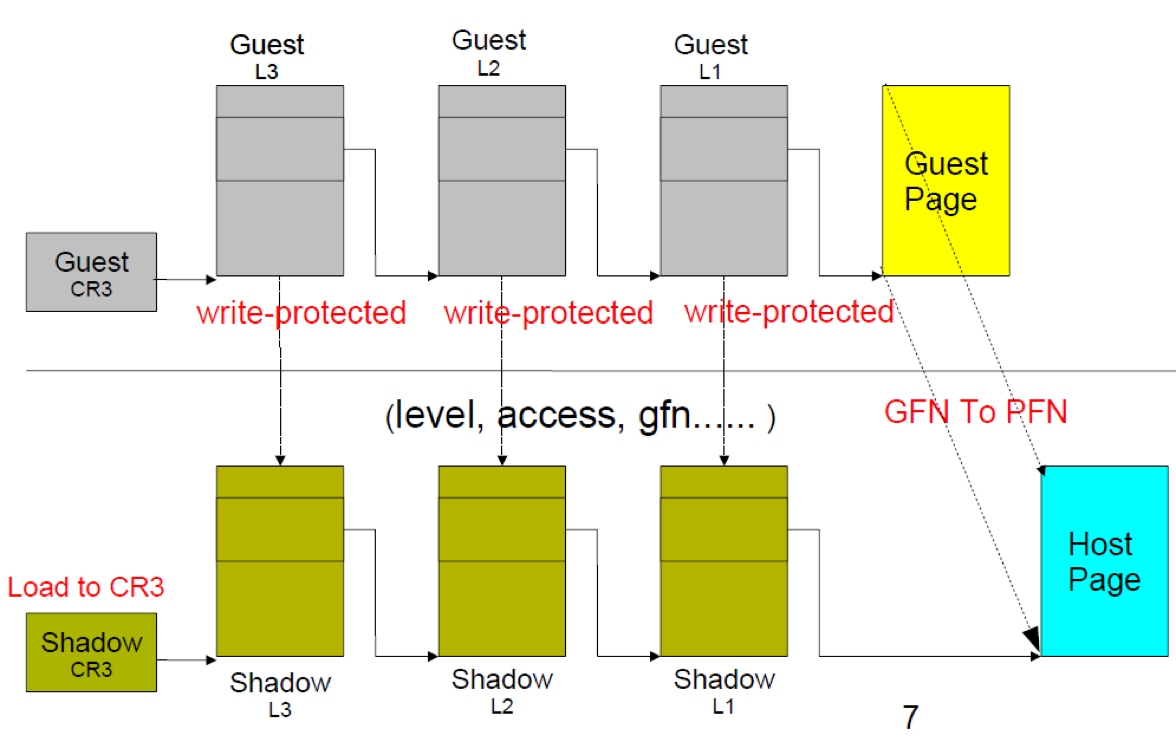
\includegraphics[width=0.4\textwidth]{spt.png}
\end{figure}

In \ref{fig1}, whenever guest OS load cr3 which is a privileged instruction, VMM will trap that and load shadow page table cr3. Since shadow page table is in write protection. Every write to shadow page table will result in a page fault. VMM will have a chance to fix the page fault and update shadow page table. After the shadow page table and the guest OS page table are synchronized, every memory access to the page returns the normal process. VMM has no aware of guest OS memory access.

In order to track guest page access, we have to mark the page table to introduce some 
artificial page fault. According to The Intel 64 and IA-32 Architectures Software Developer's Manual\cite{Intel}, there is reserved bit in PTE. For example, in our experiment environment, which is on intel x86-64 processors using IA-32e paging mode, there are four bits that is reserved (bit 51:48). \ref{fig2} Reserved bits must be 0, otherwise, the entry is used neither to reference another paging-structure entry nor to map a page. So if we have PTE collections, it's easy to track all page reference by marking reserved bits. The PTE number is a little bit huge. For a 4GB memory computer as an example, there are up to 1048576 PTEs if 4KB page used not considering huge page(2MB). An optimization is to collect page directory entry that references a page table. In x86-64 architecture, one page directory entry points to a page table that has 512 PTE. Using page directory entry(PDE) collection cuts down the space overhead to 2048 which is acceptable.
\begin{figure}\label{fig2}
	\centering
	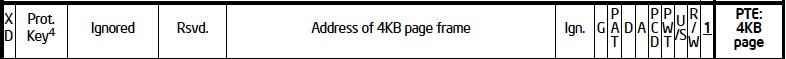
\includegraphics[width=0.4\textwidth]{pte.jpeg}
\end{figure}

\subsection{Hot page set}
With PDE collection, we have chances to track all page reference by marking reserved bit. Once the marked page is used by guest OS, it will trap into VMM. Reserved bit should be clear and then give back the execution right to guest OS. Before giving back the execution right, VMM can record the referenced page and do lru or aet calculation. After memory access is over, mark reserved bit again. However, if all memory access is tracked, machines can hardly run. There are millions of memory access every second. One page fault means cache miss, TLB miss and context switch between guest OS and VMM.

\begin{figure}\label{fig3}
	\centering
	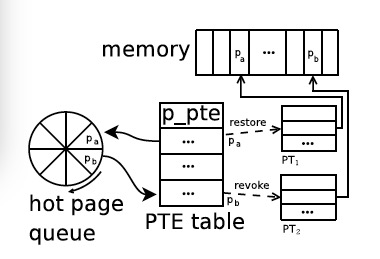
\includegraphics[width=0.4\textwidth]{hss.jpeg}
\end{figure}

Zhao\cite{Zhao2009Dynamic} first presents hot set theory. They logically divide host pages into two sets, a hot page set and a cold page set. Only accesss to cold pages are trapped. Initially, all pages are marked as cold meaning all PTE's reserved bit is set. Cold pages enters hot page set after first use and clear reserved bit. Hot page set is organized as a FIFO queue. Once a page is marked as hot, its page frame number is appended to the tail of the queue. When the queue is full, the page referred to by the head entry is degenerated to the cold set, setting reserved bit again.

Using hot page set reduces the number page faults by several orders of magnitude. The reason behind this is the program locality. Data is usually reused within a relatively small time duration. TLB is the hardware optimization for reducing the time that recent used time look up page table in memory. Due to hardware limitations, the size of TLB is small. Hot page set is stored in memory and it's a software optimization. Zhao\cite{Zhao2009Dynamic} sets hot page size up to 4096 and still has a high precision. Our work refers to their selection for the size of hot page set and the following experimental data seems it works very well.

\subsection{Sampling}
Exeperiment result show just using hot page set still produces a lot of overhead. For example, xxxxxxxxxxxxx. Another optimization needs to be taken to reduce the overhead to the normal range. Our prior works, Shards\cite{shards} and AET\cite{aet}, both uses sampling technique. Their core idea is centered around a simple question, whether they can get Approximate optimal MRC by random sampling. Although there are a lot of optimizations for lru algorithm or newly invented novel algorithm to reduce the cost on MRC construction. Sampling from the source solves the problem of overhead.

These two works of sampling have some distinctions. Shards‘ concept is pretty simple - for each referenced location L, the decision of whether or not to sample L is based on that hash(L) satisfies some condition - hash(L) mod 100\textless K means K\% sampling rate. AET sampling according to probability choose whether or not to sample a reference. It means the distance between two adjacent monitoring points is a random value. Unlike shards' method, every reference in the trace has a chance to be sampled. These two works both show good results.

In our situation, random sampling seems impossible. There is so huge overhead to get full reference to memory, not saying randomly pick some to track. What we have is a collection of PTEs. A practical way to use sample method to track page reference is randomly choosing PTE according the hash value of PTE address which is like Shards. To avoid tracking fixed set of PTE, we periodically change the sampling collection. Every period, we scan the PTE collection and randomly pick PTE to set reserved bit. In this way, we guarantee our tracking set is random and often changing.

\subsection{Dynamic sampling rate}
Hot page set and sampling reduce the overhead drastically. But there is still a problem. Hot page set size is based on locality. Programs have different degrees of locality. Even within one program, locality varies frequently. Fixed hot page set size and sampling rate may not reduce the overhead to the acceptable range. Meantime, if a program's memory needs are not so big, with a large hot page set size and a small track rate, the number of tracked page becomes too small. AET algorithm is based on probability and too small samples will also affect accuracy. Table \ref{table2} shows the overhead with fixed hot page set size(64 pages) and sampling rate($\frac{1}{128}$).

\vspace{3pt}
\renewcommand\arraystretch{1.5}
\begin{table}[H]
	\caption{Overhead}\label{table2}
	\centering
	\begin{tabular}{|c|c|}
		\hline
		benchmark & overhead \\
		\hline
		gems & 1.071972904 \\
		\hline
		milc & 1.11369509 \\
		\hline
		mcf & 1.070967742 \\
		\hline
		cactus & 1.013490725 \\
		\hline
		soplex & 1.031879195 \\
		\hline
		
	\end{tabular}
\end{table}


Increasing hot page set size or decreasing sampling rate both reduce overhead. How to make a choice, there is no theory support nor prior knowledge. It's a two viariables problem. By fixing one viarable, we change another one to watch the overhead change. Experiments result show that decreasing sampling rate reduce the overhead immediately, and increasing hot page set may or may not reduce the overhead. As shown in Table \ref{table1} We run this benchmark again to check why increasing hot page set doesn't reducing overhead immediately and count the page fault number that we manual make.

\vspace{3pt}
\renewcommand\arraystretch{1.5}
\begin{table}[H]
	\caption{GemsFDTD}\label{table1}
	\centering
	\begin{tabular}{|c|c|c|c|c|}
		\hline
		\diagbox{hss}{tr} & $\frac{1}{64}$ & $\frac{1}{128}$ & $\frac{1}{256}$ & $\frac{1}{512}$ \\
		\hline
		64 & 1.1583 & 1.0720 & 1.0415 & 1.0110 \\
		\hline
		128 & 1.1558 & 1.0771 & 1.0390 & 1.0237 \\
		\hline
		256 & 1.1507 & 1.0847 & 1.0364 & 1.0161 \\
		\hline
	\end{tabular}
\end{table}

xxxxxxx 不同热页集下page fault次数

In the tables xxxxxxx, it shows increasing hot page set size may not decreasing page fault number. The reason is that if a program's spatial locality is much larger than our hot page set size or much smaller than that, the effect of increasing hot page set size or decreasing is not evident. Keep increasing hot page set size obvious can reduce page fault numbers but this process is slow. However changing sampling rate directly reduces the size of tracking page set. Obviously it's effect is remarkable. Since we can not slow down the performance of the virtual machine, we need a machanism to reduce overhead quickly. Our research is focused on changing sampling rate. Before that, it's important to verify whether changing hot page set size or samping rate influence accuracy. From our experiment, these changes have little effect on accuracy. And from prior work, dynamic changing hot page set size is a method to reduce large working set program overhead\cite{Wang2016Dynamic}, One ten thousandth sampling rate still maintains high accuracy\cite{aet}. Based on the prior research and our experimental varify, our work use dynamic sampling rate to reduce overhead.

xxxxxx graph 精度的图

But how to change sampling rate dynamically is still a challenge. The first thing is to choose a original sampling rate. Too large or too small this value may leads to bad result. Too large sampling rate cause the overhead at the beginning too massive. And we all know adjusting sampling rate takes time. If the monitoring period is 5 seconds and it takes 6 times to adjust sampling rate to suitable value, 30 seconds are wasted. Besides that, the most severe problem is the performance of virtual machine at the tracking beginning will slow down badly which is unacceptable. Too little sampling rate also has bad effect on accuracy. Because AET is a probability algorithm, a small amount of sample will reduce the accuracy. Through experiments in our environment, we choose sampling rate of $1/128$ at first. Our virtual machine's memory configuration is 4GB, and hot page set size is 64 pages. Experiments show this sampling rate chosen controls the overall overhead at the low level. But this value still remains configurable. If virtual machine's memory is large. We suggest reducing sampling rate appropriately.

According to the experiments shown in Wang\cite{Wang2016Dynamic}, Gems, Milc and Mcf in SPEC2006 shows high overhead. We test these benchmark in our environment using 64 hot page set size and sampling rate of $1/128$.
\begin{table*}
	\centering
	\caption{这是一张奇怪的表格}\label{tab:aStrangeTable}
	\begin{tabular}{cccccc}
		\toprule
		benchmark & base time & real time & memory counter & page fault counter & overhead \\
		\midrule
		gems & 394 & 455 & 9.22331E+11 & 26517108 & 1.155800169 \\
		milc & 387 & 453 & 4.17793E+11 & 30116393 & 1.170542636 \\
		mcf & 310 & 353 & 1.46059E+11 & 17879310 & 1.138709677 \\
		\bottomrule
	\end{tabular}
\end{table*}

\section{Evaluation}
\subsection{Experimental Setup}
Our experiments are performed on an Intel CORE I7 machine with 16GB of physical memory and four 2.80 GHz cores with support of Hyper-threading(HT). All of our experiments are carried out on a hypervisor based on Xen 4.5.1 and the linux kernel version 4.2.1, while both dom0 and the guest systems are built on CentOS 6.4. To exclude the impact of CPU resource contention when multiple VMs are running, each VM is assigned a dedicated CPU core. Each VM is assigned with 4 GB of memory. And in our experiments, tracking period is 5 seconds and every 5 seconds we report the MRC curve.

Our tracking system is a general framework implementing hot page set and sampling mechanism. All kinds of algorithm can run upon that including AET model or optimized LRU. To varify AET model's accuracy, we compare the MRC curve using these two algorithm. On our online system, we use AET and LRU to calculate MRC at the same time and guarantee these two methods uses the same access trace. There are two kinds of benchmarks, one is a benchmark written on our own shown in Algorithm \ref{alg1}. We call it fake benchmark. This benchmark is pretty simple, allocate a fixed size of memory, scan this memory sequentially and repeatedly. We can control our benchmark's memory use freely. By mallocing more or less memory, we can produce even more benchmark if we like. In our experiment, each step's memory usage is as shown in table \ref{table4}. The other benchmark is from SPEC CPU 2006\cite{Henning2000spec}. These benchmark is more general and realistic and they are chosen to represent the sequential workload. 

\begin{algorithm}
	\caption{Fake benchmark}
	\label{alg1}
		\begin{algorithmic}  
			\STATE malloc N MB memory organized as an array;
			\STATE define a list L that indicates memory usage in each step;
			\FOR{each $i \in L$}  
			\STATE scan the first i MB array of N several times;\  
			\ENDFOR  
		\end{algorithmic}  
\end{algorithm}

\vspace{3pt}
\renewcommand\arraystretch{1.5}
\begin{table*}[htbp]
	\caption{Overhead}\label{table3}
	\centering
	\begin{tabular}{|c|c|c|c|c|c|c|}
		\hline
		step 1 & step2 & step3 & step4 & step5 & step6 & step7 \\
		\hline
		100MB & 300MB & 500MB & 700MB & 500MB & 300MB & 100MB \\
		\hline
	\end{tabular}
\end{table*}
\subsection{Correctness}
Hu\cite{aet} evaluates the correctness of AET using "master" MSR trace(created by \cite{Wires2014Characterizing}). The Mean Absolute Error(MAE) is 0.01 using AET random sampling with sampling rate $1*10^6$. However the "master" MSR trace is the storage traces released by Microsoft Research Cambridge(MSR)\cite{Narayanan2008Write}. They didn't evaluate AET model using real memory trace. MEB\cite{Wang2016Dynamic} using optimized LRU algorithm and hot page set gets accurate MRC curve. We compare our AET model and MEB using the same trace. How to do that is pretty simple. After tracking a page fault we manually made, we calculate this page's reuse distance by LRU list and reuse time by AET hash table. After some time, using reuse distance histogram and reuse time histogram, we can get two MRC curve by different ways. The experimental parameters are followed by MEB\cite{Wang2016Dynamic}. Hot page set size is fixed as 2048 pages. Since MEB didn't use sampling technique. In this experiment, sampling is turned off.

As shown in Figure \ref{fig4}, fake benchmark has 7 stages(size of (L) is 7). AET model uses reuse time histogram and LRU model uses reuse distance histogram. In our fake benchmark, memory is accessed sequentially. In LRU model, every access's reuse distance is the whole memory size. In AET model, we use logical time as reuse time which is the number of reference between this access and the last. So reuse time is also the whole memory size. Both reuse time histogram and the reuse distance histogram have the same shape. In this situation, we get almost the same result.

\begin{figure}[!htp]
	\caption{fake benchmark}
	\label{fig4}
	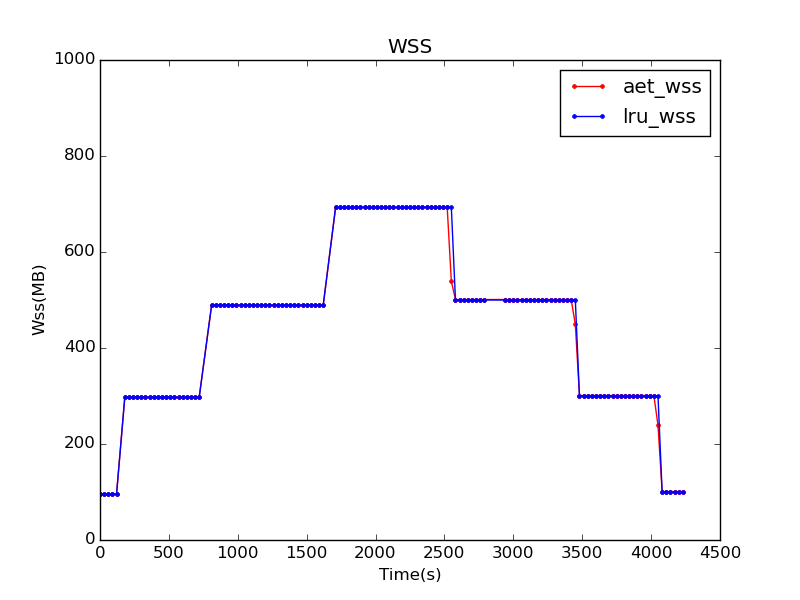
\includegraphics[width=0.5\textwidth]{img/aet_lru_cmp/aet_lru_cmp_fakestage.png}
\end{figure} 

In another situation whose memory access pattern is in real workload, we draw the miss curve by AET model and LRU model. Since our monitoring period is 5 seconds, there are too many MRC graph to show in this paper. We pick up some MRC curve randomly when running the benchmark as show in Figure \ref{fig6}. In real workload, page's reuse distance is almost less than reuse time because of the locality. Pages that are current used will be likely reused soon. AET's model obtains approximate result. With MRC curve, we can define working set easily. If we take 5\% miss rate's memory as working set, we can draw a working set changing graph. To evaluate AET model's overall accuracy, we draw working set changing graph using LRU model too. As shown in Figure \ref{fig5}, there are some errors in AET model.

Besides drawing pictures to compare the result using the two algorithm. We also calculate the Mean Absolute Error(MAE) of all SPEC 2006 benchmark. It gives about 0.01 average MAE which is good for online tracking.

\begin{figure}
	\centering
	\caption{mrc}
	\label{fig6}
	\subfigure{
		\begin{minipage}[b]{0.2\textwidth}
			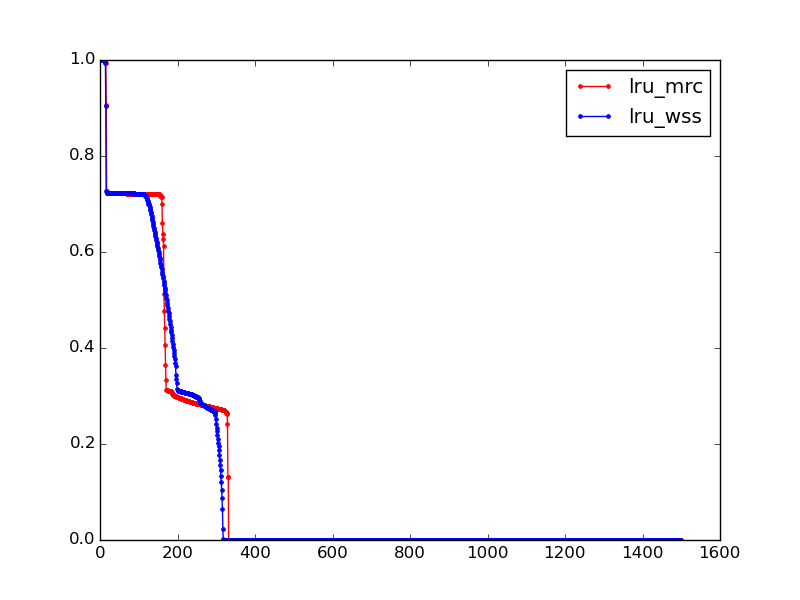
\includegraphics[width=1\textwidth]{img/mrc_cmp/mrc_cmp_fullmilc_1491919033.png} \\
			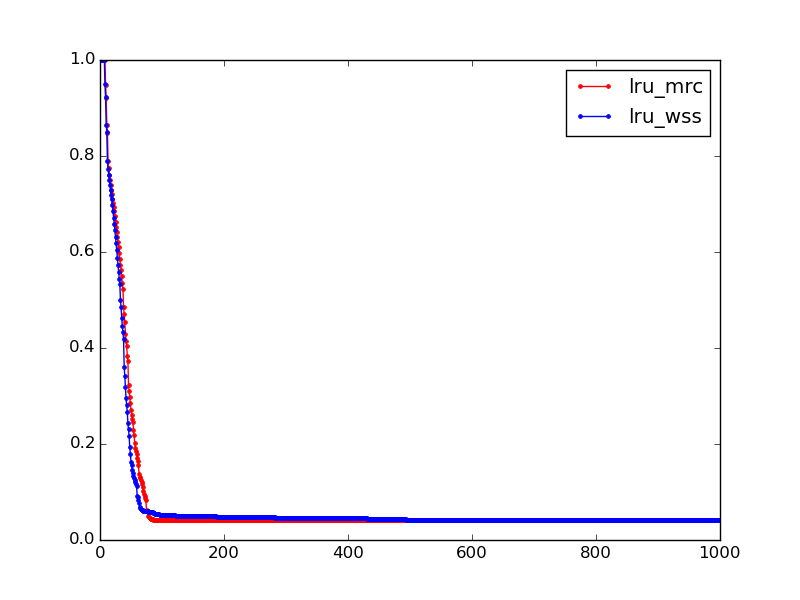
\includegraphics[width=1\textwidth]{img/mrc_cmp/mrc_cmp_fullgcc_1491926637.png} \\
		\end{minipage}
		\begin{minipage}[b]{0.2\textwidth}
			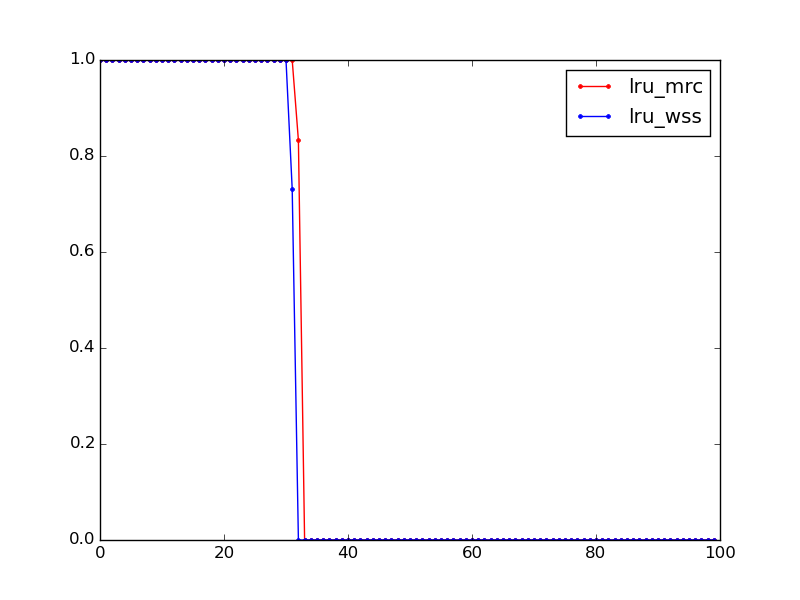
\includegraphics[width=1\textwidth]{img/mrc_cmp/mrc_cmp_fulllib_1491934003.png} \\
			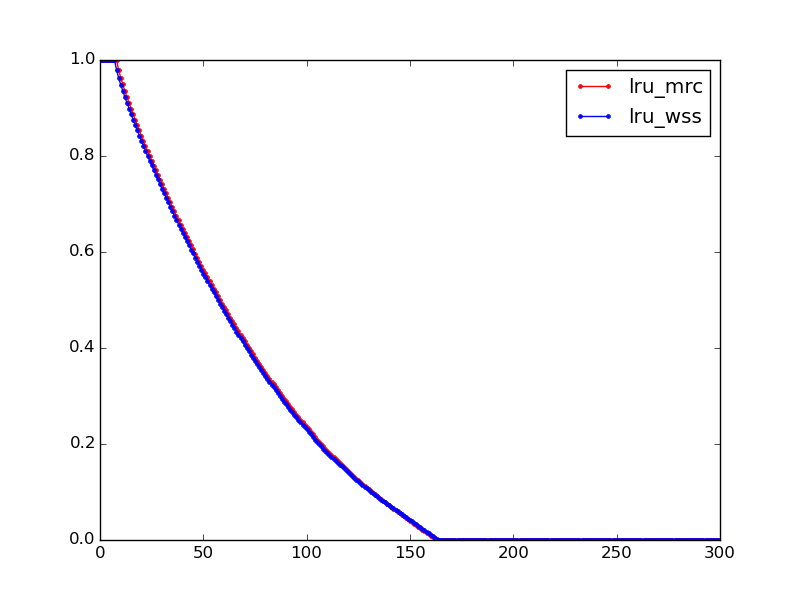
\includegraphics[width=1\textwidth]{img/mrc_cmp/mrc_cmp_fullsjeng_1491930705.png} \\
		\end{minipage}
	}
\end{figure}

\begin{figure}[!htbp]
	\centering
	\caption{wss}
	\label{fig5}
	\subfigure{
		\begin{minipage}[b]{0.2\textwidth}
			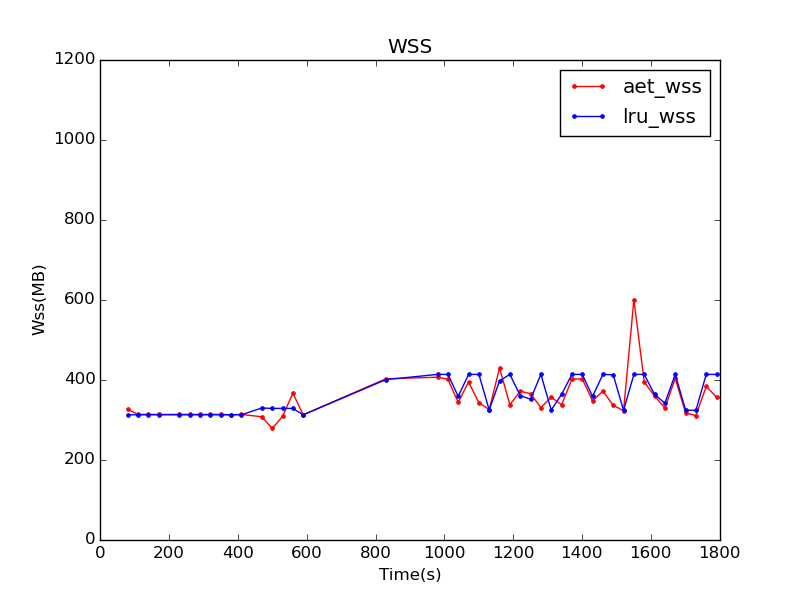
\includegraphics[width=1\textwidth]{img/aet_lru_cmp/aet_lru_cmp_milc.png} \\
			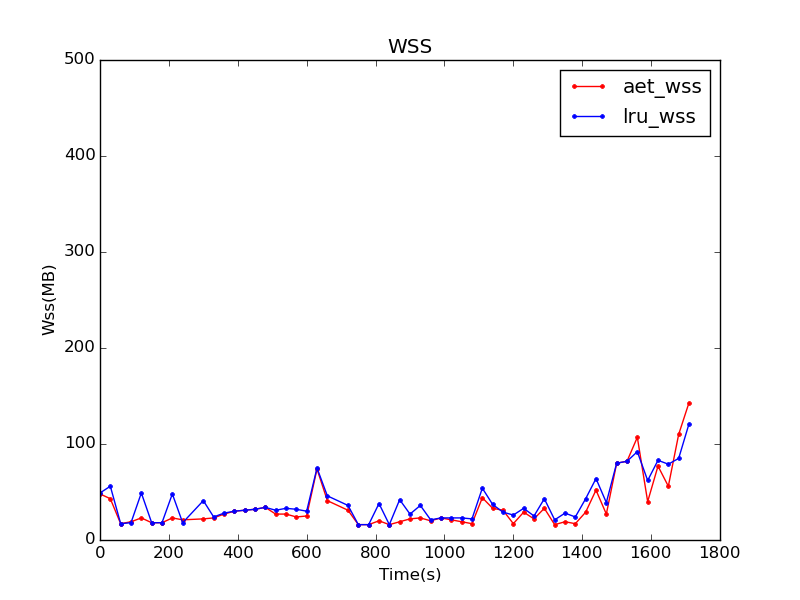
\includegraphics[width=1\textwidth]{img/aet_lru_cmp/aet_lru_cmp_gcc.png} \\
		\end{minipage}
	}
	\subfigure{
		\begin{minipage}[b]{0.2\textwidth}
			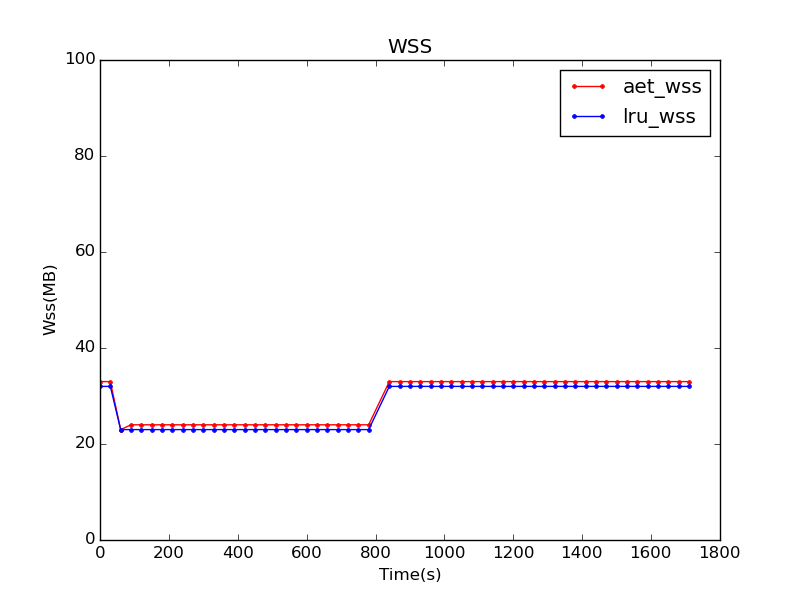
\includegraphics[width=1\textwidth]{img/aet_lru_cmp/aet_lru_cmp_lib.png} \\
			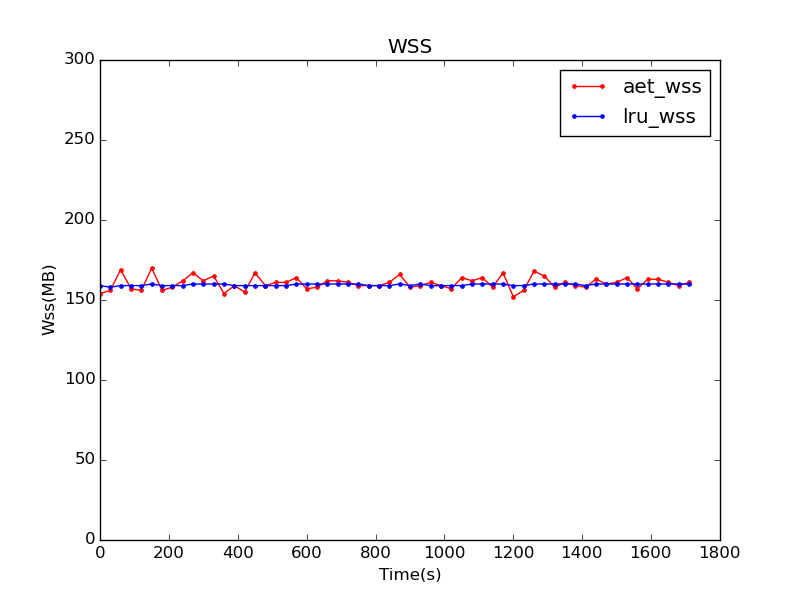
\includegraphics[width=1\textwidth]{img/aet_lru_cmp/aet_lru_cmp_sjeng.png} \\
		\end{minipage}
	}
\end{figure}

%However, comparison above doesn't use sampling technique. Sampling is the core method to reduce the overhead. Since we have evaluate our system's accurace without sampling. We just need to compare the result that uses sampling or not. The time to run benchmark is much different whether we use sampling or not. So it's hard to draw the working set trend graph in one picture or calculating MAE. We use a rough way to compare sampling result by putting all the graph in a row. The graph is as show in Figure \ref{fig7}

\begin{figure}[!htp]
	\caption{fake benchmark}
	\label{fig7}
	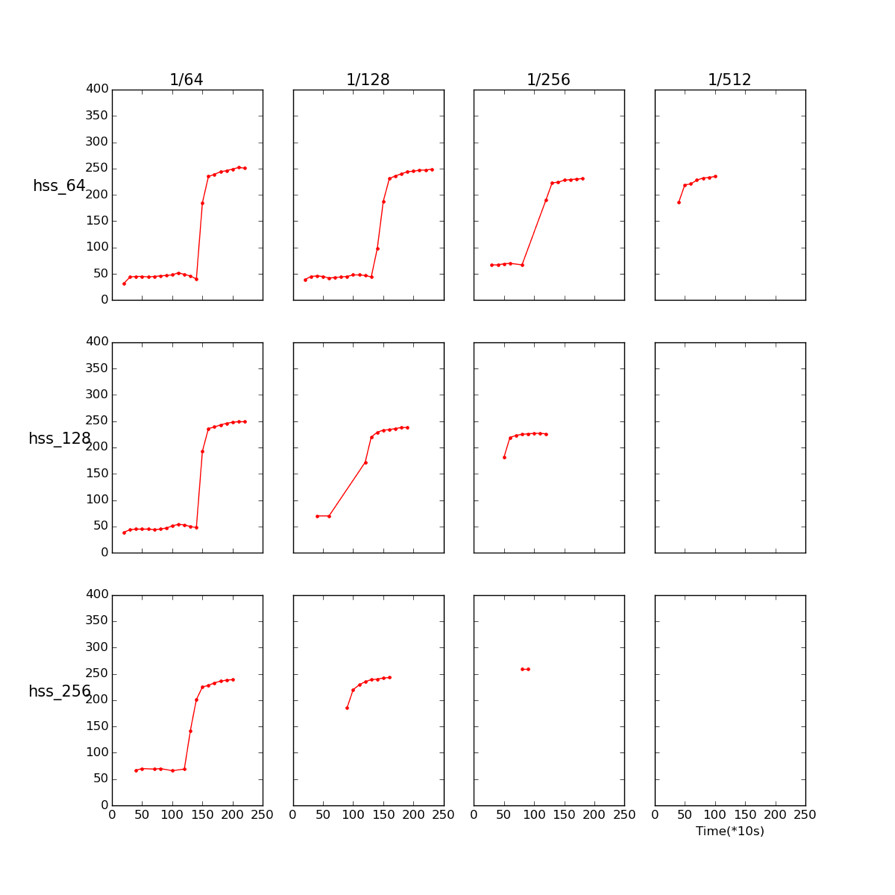
\includegraphics[width=0.5\textwidth]{img/sampling_exp/sampling_exp_milc.png}
\end{figure} 

\subsection{Fixed Sampling}
The overhead only using hot page set technique is not acceptable. We have evaluated our system with only hot page set optimization. MCF shows even 10 times overhead. And there are xx times overhead on average. We add timing program in our implementation. The first one path that consumes time in our system is the time when a page fault we created is tracked, we need to insert into a hash table, obtain reuse time and update reuse time histogram. The other one path is the time that we set PTE to manually introduce page fault. In this procedure, we have to scan all PTE, check the PTE validation and mark a bit in PTE. We periodly scan the PTE collections to make our tracking page fresh. If we have 4GB memory, Theoretically, the number of PTEs is up to 1 million so the overhead is the same as to scan an array with one million entrys. The third part of overhead is the time that collects PTE. We have optimize this process by collecting L1 page frames which contains 512 PTEs in 64 bits machine or 1024 PTEs in 32 bits machines. In another word, it reduces the space that needs to store the PTEs from one million to several thousands. When virtual machine's page is first used, we check whether its L1 page frame is stored. If not, add this frame in an array. We use hash to reduce the checking time to constant time. These three critical path is our algorithm overhead. The last overhead, the context switch time from virtual machine to VMM can not be recored and this part in our experiment is the most consuming one. We measure this overhead by watching page fault count. The number of page fault and the context switch time have positive correlations.

Using hot page set size 2048 pages without sampling , we get the table \ref{table1}. The first three factors have tiny impact on the overhead. It relects that the AET model has low calculation complexity. The most consuming part is the context switch time. The page fault number it produces under our monitor is tens of thousands of times of the one that produces in real world.

Using sampling, we can reduce the number of tracked pages. In experiments, we use 64 hot page set size and $\frac{1}{128}$ sampling rate to balance overhead and accuracy.

\section{Conclusion}



\bibliographystyle{abbrv}
\bibliography{biblio}

\end{document}


